\documentclass{article}
\usepackage{subfigure}
\usepackage{multicol}
\usepackage{graphicx}
\usepackage[utf8]{inputenc}
\usepackage[margin=.5in]{geometry}
\addtolength{\topmargin}{.875in}
\usepackage{xcolor}
\usepackage{titlesec}
\titleformat{\section}[block]{\color{black}\Large\bfseries\filcenter}{}{1em}{}
\pagestyle{headings}
\markright{toss}
\begin{document}

\section{Modeled Position}
\begin{figure}[h!]
\begin{multicols}{2}
    \includegraphics[scale=0.6]{/Users/CoraJune/Documents/GitHub/Pozyx/new_models/toss/figures/position_model/redBall.png}
    \includegraphics[scale=0.6]{/Users/CoraJune/Documents/GitHub/Pozyx/new_models/toss/figures/position_model/yellowBall.png}
\end{multicols}

\begin{multicols}{2}
    \includegraphics[scale=0.6]{/Users/CoraJune/Documents/GitHub/Pozyx/new_models/toss/figures/position_model/blueBall.png}
    \includegraphics[scale=0.6]{/Users/CoraJune/Documents/GitHub/Pozyx/new_models/toss/figures/position_model/orangeBall.png}
\end{multicols}


\end{figure}
\newpage
%%%%%%%%%%%%%%%%%%%%%%%%%%%%%%%%%%%%%%%%%%%%%%%%%%%%%%%%%%%%%%%%%%%%%%%%%%%%%%%%%%%%%%%%%%%%%%%%%%%%%%%%%%%%%%%%%%
\markright{toss}
\section{Modeled Velocity}
\begin{figure}[h!]
\begin{multicols}{2}
    \includegraphics[scale=0.6]{/Users/CoraJune/Documents/GitHub/Pozyx/new_models/toss/figures/velocity_model/redBall.png}
    \includegraphics[scale=0.6]{/Users/CoraJune/Documents/GitHub/Pozyx/new_models/toss/figures/velocity_model/yellowBall.png}
\end{multicols}

\begin{multicols}{2}
    \includegraphics[scale=0.6]{/Users/CoraJune/Documents/GitHub/Pozyx/new_models/toss/figures/velocity_model/blueBall.png}
    \includegraphics[scale=0.6]{/Users/CoraJune/Documents/GitHub/Pozyx/new_models/toss/figures/velocity_model/orangeBall.png}
\end{multicols}

\end{figure}
\newpage
%%%%%%%%%%%%%%%%%%%%%%%%%%%%%%%%%%%%%%%%%%%%%%%%%%%%%%%%%%%%%%%%%%%%%%%%%%%%%%%%%%%%%%%%%%%%%%%%%%%%%%%%%%%%%%%%5%
\markright{toss}
\section{Modeled Acceleration}
\begin{figure}[h!]
\begin{multicols}{2}
    \includegraphics[scale=0.6]{/Users/CoraJune/Documents/GitHub/Pozyx/new_models/toss/figures/acceleration_model/redBall.png}
    \includegraphics[scale=0.6]{/Users/CoraJune/Documents/GitHub/Pozyx/new_models/toss/figures/acceleration_model/yellowBall.png}
\end{multicols}

\begin{multicols}{2}
    \includegraphics[scale=0.6]{/Users/CoraJune/Documents/GitHub/Pozyx/new_models/toss/figures/acceleration_model/blueBall.png}
    \includegraphics[scale=0.6]{/Users/CoraJune/Documents/GitHub/Pozyx/new_models/toss/figures/acceleration_model/orangeBall.png}
\end{multicols}

\end{figure}
\newpage
%%%%%%%%%%%%%%%%%%%%%%%%%%%%%%%%%%%%%%%%%%%%%%%%%%%%%%%%%%%%%%%%%%%%%%%%%%%%%%%%%%%%%%%%%%%%%%%%%%%%%%%%%%%%%%%%%%
\markright{toss}
\section{Modeled Drag Force}
\begin{figure}[h!]
\begin{multicols}{2}
    \includegraphics[scale=0.6]{/Users/CoraJune/Documents/GitHub/Pozyx/new_models/toss/figures/dragForce_model/redBall.png}
    \includegraphics[scale=0.6]{/Users/CoraJune/Documents/GitHub/Pozyx/new_models/toss/figures/dragForce_model/yellowBall.png}
\end{multicols}

\begin{multicols}{2}
    \includegraphics[scale=0.6]{/Users/CoraJune/Documents/GitHub/Pozyx/new_models/toss/figures/dragForce_model/blueBall.png}
    \includegraphics[scale=0.6]{/Users/CoraJune/Documents/GitHub/Pozyx/new_models/toss/figures/dragForce_model/orangeBall.png}
\end{multicols}

\end{figure}
\newpage
%%%%%%%%%%%%%%%%%%%%%%%%%%%%%%%%%%%%%%%%%%%%%%%%%%%%%%%%%%%%%%%%%%%%%%%%%%%%%%%%%%%%%%%%%%%%%%%%%%%%%%%%%%%%%%%%%55%
\markright{toss}
\section{Fitting Routine Open}
\begin{figure}[h!]
\begin{multicols}{2}
    \includegraphics[scale=0.6]{/Users/CoraJune/Documents/GitHub/Pozyx/new_models/toss/figures/fitting/redBall.png}
    \includegraphics[scale=0.6]{/Users/CoraJune/Documents/GitHub/Pozyx/new_models/toss/figures/fitting/yellowBall.png}
\end{multicols}

\begin{multicols}{2}
    \includegraphics[scale=0.6]{/Users/CoraJune/Documents/GitHub/Pozyx/new_models/toss/figures/fitting/blueBall.png}
    \includegraphics[scale=0.6]{/Users/CoraJune/Documents/GitHub/Pozyx/new_models/toss/figures/fitting/orangeBall.png}
\end{multicols}


\end{figure}

%%%%%%%%%%%%%%%%%%%%%%%%%%%%%%%%%%%%%%%%%%%%%%%%%%%%%%%%%%%%%%%%%%%%%%%%%%%%%%%%%%%%%%%%%%%%%%%%%%%%%%%%%%%%%%%%%%
\end{document}

